\subsection{Self-Trapped Excitons}

Thermal fluctuations induce slight lattice vibrations that act as a trigger, creating a transient local deformation. The strongly localized exciton is captured by this distortion. Through massive exciton-phonon coupling, it abruptly discharges its potential energy into the lattice, considerably deepening the local potential well, shown schematically in Figure~\ref{fig:STE}.

\begin{figure}[ht]
\centering
\begin{tikzpicture}[scale=1.0]

%-------------------------------------------------
% Axes
%-------------------------------------------------
\draw[-stealth,thick] (-3.7,0) -- (5.7,0)
node[right]{Coordination coordinate $Q$};

\draw[-stealth,thick] (-3.5,-0.2) -- (-3.5,7.6)
node[above]{Energy};

%-------------------------------------------------
% Ground state
%-------------------------------------------------
\draw[very thick]
plot[smooth] coordinates{
(-3.0,1.8)
(-2.0,0.9)
(-1.0,0.25)
(0.0,0.0)
(1.0,0.25)
(2.0,0.9)
(3.0,1.8)
(4.0,3.0)
(5.0,4.3)
};

\node[below left] at (7.5,4){Valence Band};

%-------------------------------------------------
% Excited state
%-------------------------------------------------
\draw[very thick]
plot[smooth] coordinates{
(-2.8,6.9)
(-2.0,5.8)
(-1.0,4.9)
(0.0,4.5)
(1.0,5.2)
(2.0,5.8)
(3.0,5.0)
(4.0,4.0)
(5.0,5.5)
};

\node[left] at (8,6){Conduction Band};

%-------------------------------------------------
% FE -> STE relaxation
%-------------------------------------------------
\draw[dashed,thick,->]
(1.6,6)
to[out=0,in=120]
(3.8,5);

%-------------------------------------------------
% Optical excitation
%-------------------------------------------------
\draw[ultra thick,blue,-stealth]
(0,0) -- (0,4.5);

%-------------------------------------------------
% Radiative emission
%-------------------------------------------------
\draw[ultra thick,red,-stealth]
(4.0,4.0) -- (4.0,3);

%-------------------------------------------------
% Photon symbols
%-------------------------------------------------
\draw[blue,thick,decorate,
decoration={snake,amplitude=1.5pt,segment length=4pt}]
(-1.6,2.8)--(0,2.8);

\draw[red,thick,decorate,
decoration={snake,amplitude=1.5pt,segment length=4pt}]
(2.7,3.5)--(4,3.5);

%-------------------------------------------------
% Labels
%-------------------------------------------------
% Recombinaison radiative
% Photon incident

% Petite pointe de flèche
\draw[blue,-{Stealth[length=2.8mm,width=2mm]},line width=1.2pt]
(0,2.8)--(0.1,2.8);
\draw[red,-{Stealth[length=2.8mm,width=2mm]},line width=1.2pt]
(2.7,3.5)--(2.6,3.5);
%-------------------------------------------------
% FE minimum
%-------------------------------------------------
\fill[blue] (0,4.5) circle (2.2pt);

% STE minimum
\fill[red] (4.0,4.0) circle (2.2pt);

\end{tikzpicture}
\caption{Configuration-coordinate diagram illustrating the formation of a self-trapped exciton (STE). After photoexcitation, a free exciton relaxes non-radiatively through lattice distortion into the STE configuration before radiative recombination.}
\label{fig:STE}
\end{figure}


This intense localized energy weakens and breaks the $\text{Si--O--Si}$ covalent bond, displacing the oxygen atom from its equilibrium position. This structural rupture generates two dangling bonds, each holding an unpaired electron. In this strongly distorted configuration, the exciton self-traps. The hole localizes on the oxygen dangling bond, while the electron remains bound to the silicon dangling bond~\cite{mao2004}, as sketched in Figure~\ref{fig:dangling_bonds}.

\begin{figure}[h!]
    \centering
    \begin{subfigure}{0.46\textwidth}
        \centering
        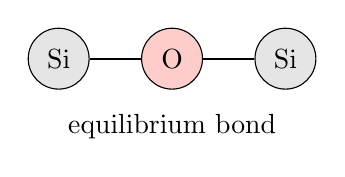
\begin{tikzpicture}[scale=0.9]
            \node[circle, draw, fill=gray!20, minimum size=22pt] (Si1) at (0,0) {Si};
            \node[circle, draw, fill=red!20, minimum size=22pt] (O)   at (1.6,0) {O};
            \node[circle, draw, fill=gray!20, minimum size=22pt] (Si2) at (3.2,0) {Si};
            \draw[thick] (Si1) -- (O);
            \draw[thick] (O) -- (Si2);
            \node[below] at (1.6,-0.65) {equilibrium bond};
        \end{tikzpicture}
        \caption{Before: intact $\text{Si--O--Si}$ bridge, oxygen at its equilibrium position.}
    \end{subfigure}
    \hfill
    \begin{subfigure}{0.46\textwidth}
        \centering
        \begin{tikzpicture}[scale=0.9]
            \node[circle, draw, fill=gray!20, minimum size=22pt] (Si1) at (0,0) {Si};
            \node[circle, draw, fill=red!20, minimum size=22pt] (O)   at (2.3,0.9) {O};
            \node[circle, draw, fill=gray!20, minimum size=22pt] (Si2) at (3.2,0) {Si};
            \draw[thick] (O) -- (Si2);
            \draw[thick, dashed, gray] (Si1) -- (O);
            \draw[kfcol, thick] (Si1) -- ++(-0.75,-0.55);
            \filldraw[kfcol] ($(Si1)+(-0.75,-0.55)$) circle (2.2pt);
            \node[kfcol, below] at ($(Si1)+(-0.75,-0.75)$) {\footnotesize electron};
            \draw[qcol, thick] (O) -- ++(-0.15,0.85);
            \node[qcol] at ($(O)+(-0.15,1.05)$) {\footnotesize $+$};
            \node[qcol, above] at ($(O)+(-0.15,1.2)$) {\footnotesize hole};
        \end{tikzpicture}
        \caption{After: the Si--O bond breaks, the oxygen relaxes off site, leaving a silicon dangling bond carrying the electron and an oxygen dangling bond carrying the hole.}
    \end{subfigure}
    \caption{Schematic bond-breaking mechanism of self-trapping in $\mathrm{SiO}_2$, simplified to a linear $\text{Si--O--Si}$ fragment for clarity (the real network is tetrahedrally coordinated). The two dangling bonds left behind are the microscopic identity of the self-trapped exciton.}
    \label{fig:dangling_bonds}
\end{figure}

This mechanism is responsible for the formation of Self-Trapped Excitons in silica. The excitation energy is rapidly converted into local lattice distortion and permanent structural modifications of the material~\cite{mao2004}.
